\section{Экспериментальное исследование}

Для экспериментальной проверки разработанного программного средства были проведены две серии экспериментов. Первая серия проведена для сравнения разработанного программного средства с наивным байесовским классификатором, используемым во многих открытых системах фильтрации спама. Кроме того, было произведено сравнение с байесовским классификатором из системы dspam, использующего методы, описанные в \cite{ROBINSON} . Серия призвана показать, что разработанное средство работает не хуже байесовских методов.

Вторая серия экспериментов проведена для проверки работы системы в многопрофильном режиме.

\subsection{Сравнение с наивным байесовским классификатором и байес-подобным классификатором из dspam}

\subsubsection {Набор данных}

Тестирование производилось на двух публичных наборах email-сообщений.

\begin{enumerate}
	\item SpamAssassin public corpus \cite{SAPC}
	\item CEAS 2008 Live Spam Challenge Laboratory Corpus \cite{CEAS}
\end{enumerate}

\subsubsection{Методика тестирования}

Тестирование производилось с использованием метода скользящего контроля: выборка разбивалась на пять частей, на четырех из которых проводилось обучение, а на пятой - контроль. Выборка \cite{CEAS} ввиду своей большой величины была разделена на несколько частей, на каждой из которых тестирование было произведено отдельно. 

Результат тестирования представлен в виде графика соответствия величин вероятности ложно-положительного срабатывания и вероятности верного обнаружения спама. Точка на графике обозначает что при определенной границе решающего правила система будет работать именно в таком режиме: фильтровать спам с вероятностью показанной на оси ординат и классифицировать легитимные письма как спам с вероятностью показанной на оси абсцисс. Чем выше проходит график, тем более качественно работает система фильтрации.

\subsubsection{Результаты тестирования}
На графике \ref{SAPCBAYESSVM}  представлен результаты тестирования на наборе \cite{SAPC}. Видно, что разработанное средство всегда работает лучше чем наивный байесовский классификатор.

Байесовский классификатор из системы dspam показывает примерно такие же результаты, что и разработанный метод.
\begin{figure}[h]
\begin{center}
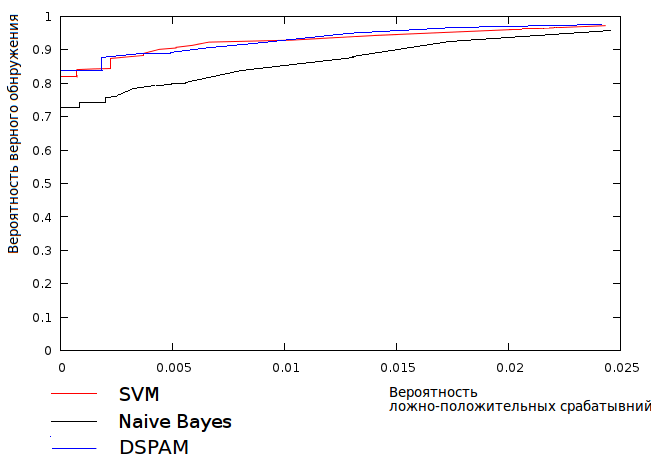
\includegraphics[width=15cm]{img/graphic}
\end{center}
\caption{Сравнение качества тестирования реализованного алгоритма, наивного байесовского классификатора на наборе\cite{SAPC}}
\label{SAPCBAYESSVM}
\end{figure}

Тестирование на наборе \cite{CEAS} дало аналогичный же результат.

\subsection{Тестирование работы в многопрофильном режиме}

\subsubsection{Набор данных}
Тестирование производилось на наборе данных SpamAssassin Public Corpus \cite{SAPC}.
Для проведения эксперимента сообщения, представленные в выборке были разделены на 3 класса:
\begin{enumerate}
\item Класс, сообщения из которого все письма считаются легитимной почтой.
\item Класс, сообщения из которого все пользователи считают спамом
\item Класс, сообщения из которого считают спамом некоторые из пользователей
\end{enumerate}

В класс 1 были включены все сообщения, отмеченные в наборе \cite{SAPC} как спам. Классы 2 и 3 были получены из писем, отмеченных в наборе \cite{SAPC} как легитимная почта путем кластеризации (метод кластеризации описан в \cite{ROZ})
\begin{enumerate}
	\item Эксперимент показывающий что многопрофильность работает, и обучение на данных одного пользователя распространяется на другого. Сообщения из всех трех классов были случайным образом разделены на две части (для первого и второго пользователей). Обучение производилось на всех трех наборах для первого пользователя и на первых двух для второго. Далее было произведено тестирование пользователей на сообщениях из третьей группы и посчитаны оценки вероятности принадлежности к спаму для писем. На результирующем графике показаны диапазоны вероятности и количество писем попавших в этот диапазон для каждого из пользователей.

	\item Эксперимент показывающий что разное мнение пользователей о группе писем не приводит к проблемам. Для этого сообщения из всех трех классов были поделены случайным образом на три части (по одной части для трех тестовых пользователей). Для всех трех пользователей было произведено обучение на выборке из первого класса как на спаме, на выборке из второго класса как на легитимной почте. Дополнительно для первого пользователя было произведено обучение на выборке из третьего класса как на легитимной почте, для второго пользователя как на спаме, для третьего обучение на третьем классе не производилось. Тестирование производилось на контрольной выборке писем из третьего класса. На результирующем графике для каждого пользователя показаны диапазоны вероятности и количество писем попавших в этот диапазон.
	
\end{enumerate}
\subsubsection{Результаты тестирования}
На графиках представлены результаты тестирования работы средства в многопрофильном режиме. 

Из графика \ref{EXPERIMENT2} видно, что обучение на одном пользователе распространяется на другого пользователя.

Из графика \ref{EXPERIMENT3} видно, что если мнения пользователей о каком-то классе писем различны, то система так же будет работать корректно. При этом если мнения пользователей о классе писем различаются, то для пользователя, который еще не добавлял писем из этого класса в обучающую выборку система будет выдавать некоторые промежуточные оценки.

\begin{figure}[h]
\begin{center}
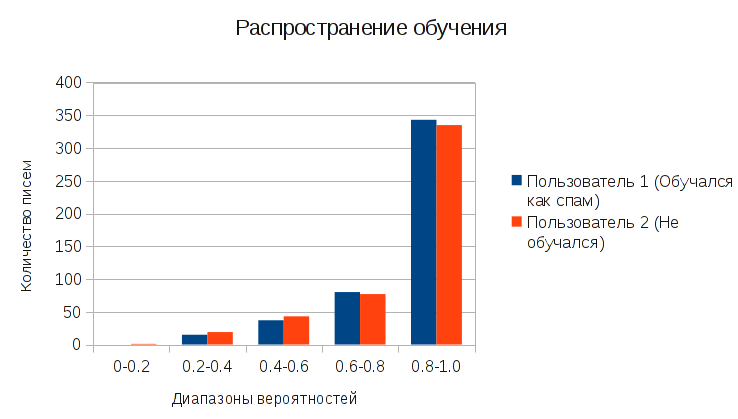
\includegraphics[width=15cm]{img/experiment2}
\end{center}
\caption{Результаты тестирования пользователя на третьем тестовом наборе. Обучение было произведено на другом пользователе \cite{SAPC}}
\label{EXPERIMENT2}
\end{figure}

\begin{figure}[h]
\begin{center}
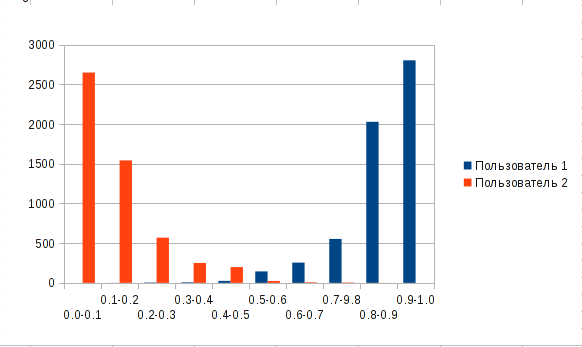
\includegraphics[width=15cm]{img/experiment3}
\end{center}
\caption{Результаты тестирования на третьем тестовом наборе после обучения на данных из этого набора первого и второго пользователя.}
\label{EXPERIMENT3}
\end{figure}


\subsection{Производительность}
Для проверки производительности метода были произведены замеры времени добавления писем в выборку, времени генерации модели и время, которое занимает классификация писем. Кроме того, для сравнения, аналогичные замеры были произведены для стандартного байесовского классификатора, включенного в систему dspam. Стадия построения модели для байесовских алгоритмов отдельно не выделяется, поэтому для dspam такие замеры произведены не были.

Были произведены замеры времени добавления и построения моделей для 20 (10 спам + 10 легитимная почта), 200 (100 спам + 100 легитимная почта),  и 2000 (1000 спам + 1000 легитимная почта) сообщений.

Для каждой построенной модели были произведены замеры времени классификации n/2 сообщений (где n - размер выборки). 

Результаты замеров  времени добавления в писем в модель, а также  времени генерации модели  представлены на графике \ref{EXLEARNING}

\begin{figure}[h]
\begin{center}
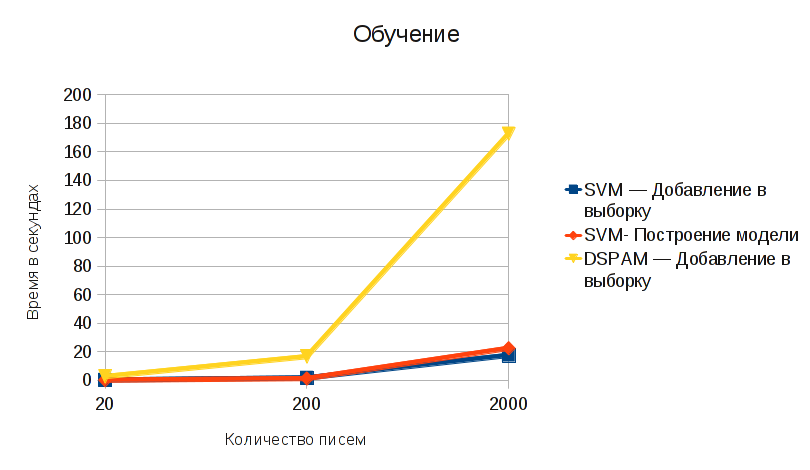
\includegraphics[width=15cm]{img/learn}
\end{center}
\caption{Замеры времени обучения и генерации модели. Разработанное средство работает эффективнее стандартного алгоритма из системы dspam}
\label{EXLEARNING}
\end{figure}


Результаты замеров времени классификации представлены на графике \ref{EXTESTING}
\begin{figure}[h]
\begin{center}
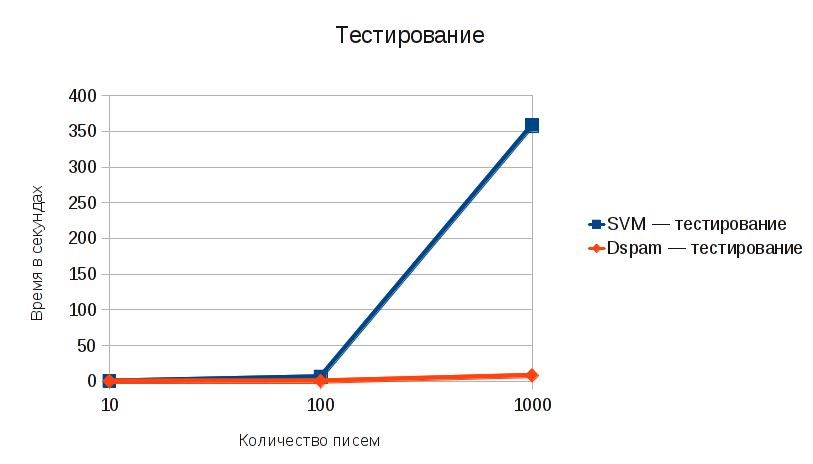
\includegraphics[width=15cm]{img/testing}
\end{center}
\caption{Замеры времени классификации. Стандартный dspam эффективнее разработанного средства}
\label{EXTESTING}
\end{figure}

